%profilingresults
Figure \ref{fig:sfda} shows the profiling results for the throughput of 
VP at different CPU-GPU allocations of the 3 tasks and different frequencies of the CPU and the GPU. 
Note, the CPU can be clocked upto 2.32 GHz (on all 4 cores), while the GPU can be clocked upto 0.852 GHz. 
We select 6 operating frequencies evenly spaced from the minimum and maximum Jetson CPU and GPU frequencies for both the CPU and the GPU. 

\begin{figure}[htbp]
	\centering
	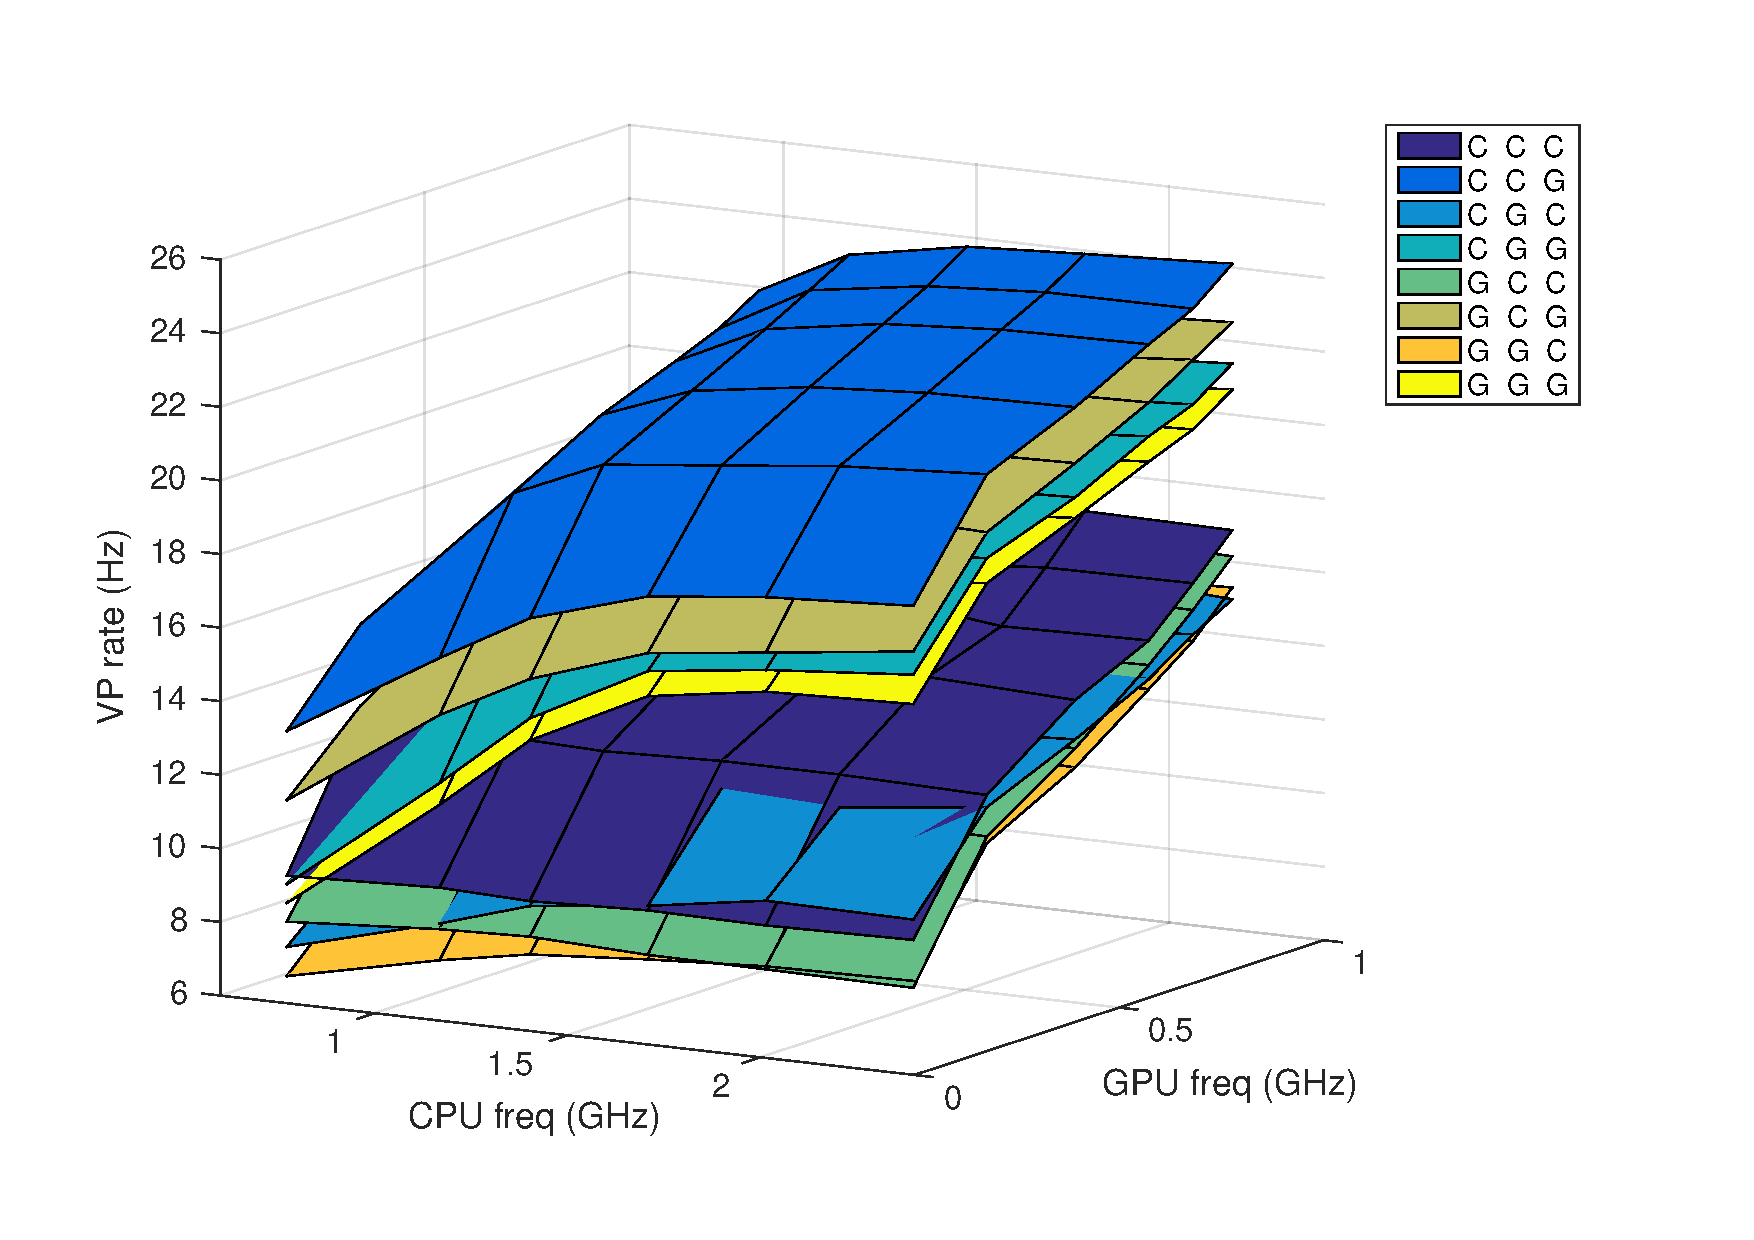
\includegraphics[width=0.46\textwidth]{Figs/surf_Rate.pdf}
	\caption{VP throughput. Each surface corresponds to a particular schedule (see legend). For a given schedule, different CPU and GPU frequencies yields a different throughput. (Color in online version).}
	\label{fig:sfda}%same freq diff assignment}
\end{figure}

%\begin{figure}[hbtp]
%\centering
%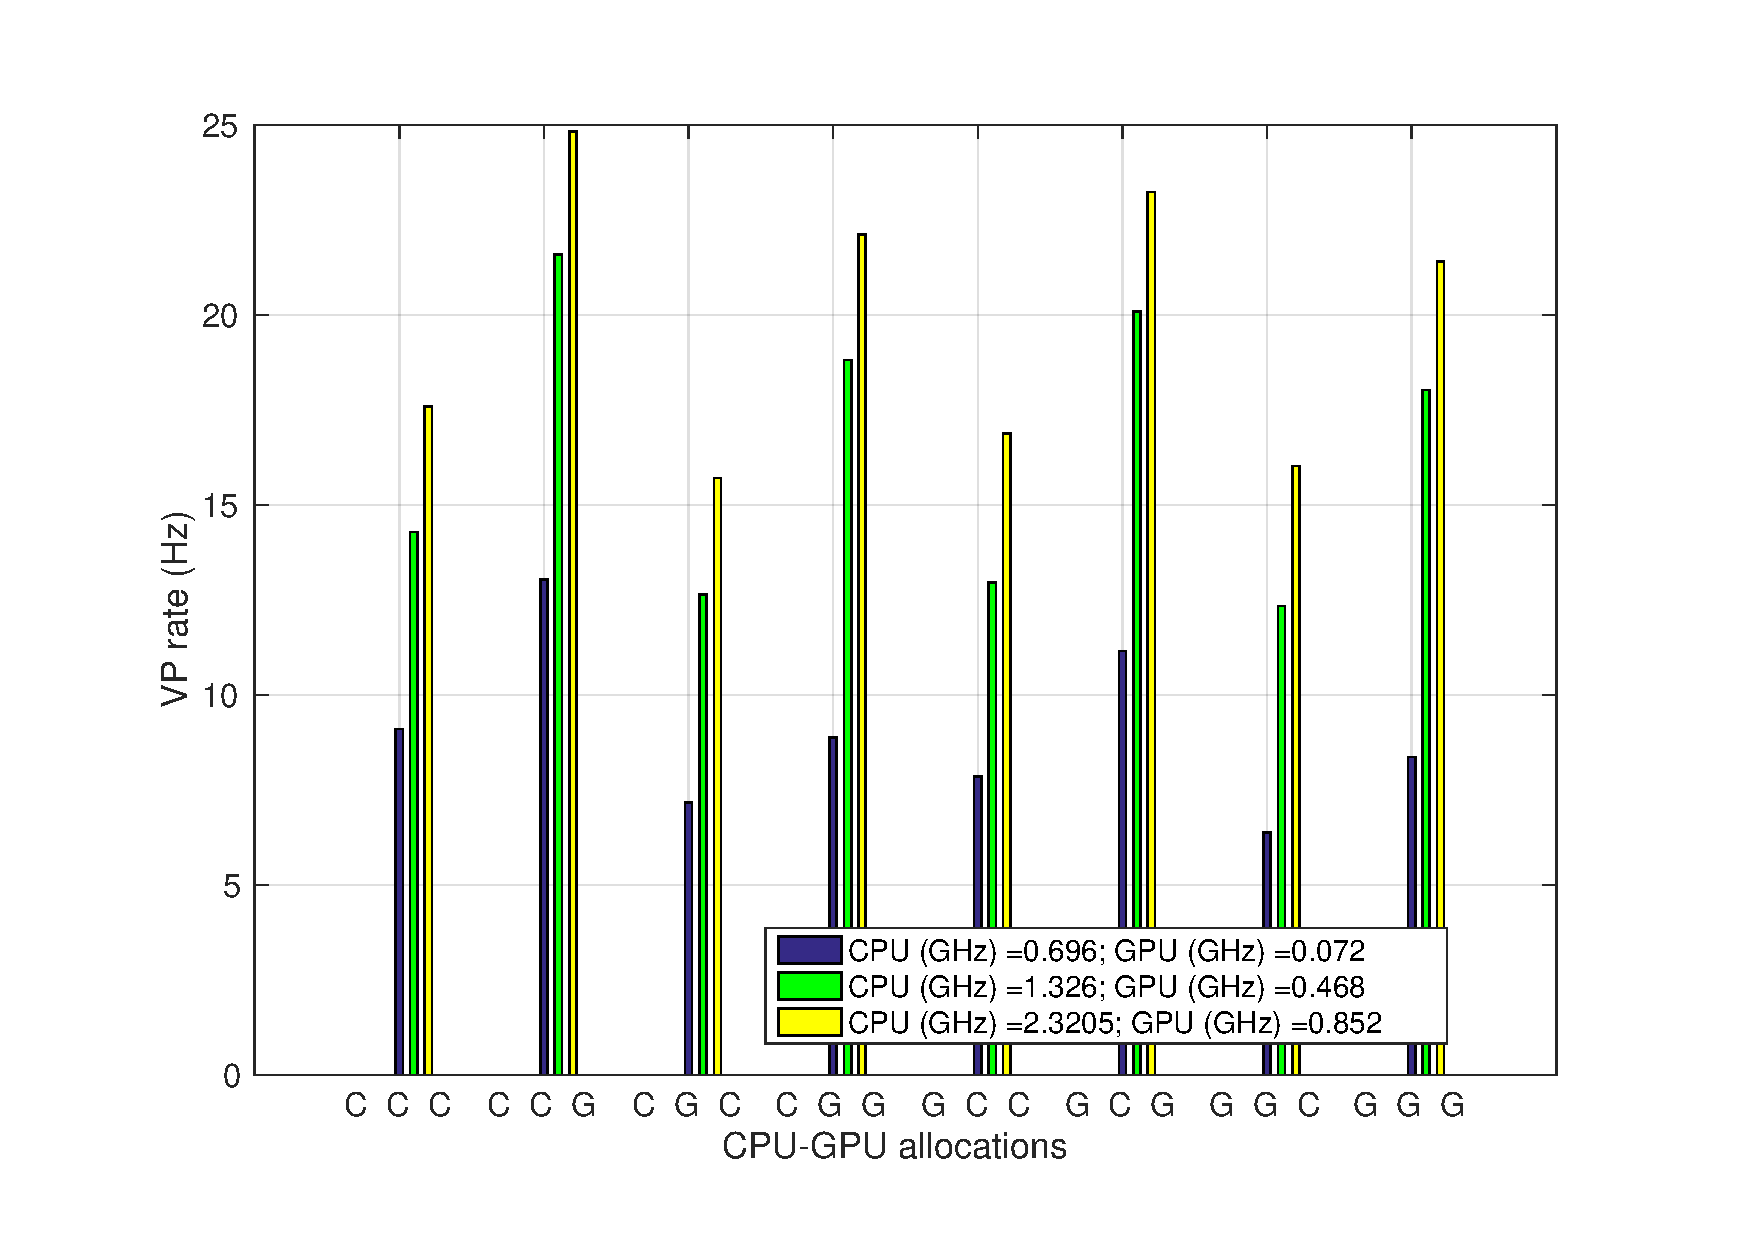
\includegraphics[scale=0.3]{Figs/RateHist.pdf}
%\caption{Control update rate for different frequencies and a given CPU-GPU assignment. For clarity we only consider 3 CPU and GPU frequencies for this %figure, ranging from the minimum to the maximum of frequencies of CPU and GPU. (Color in online version) }
%\label{fig:dfsa} %diff freq same assignment}
%\end{figure}

Figure \ref{fig:sfda_pow} shows the profiling of average power consumed by VP over all frames in the video.


\begin{figure}[htbp]
	\centering
	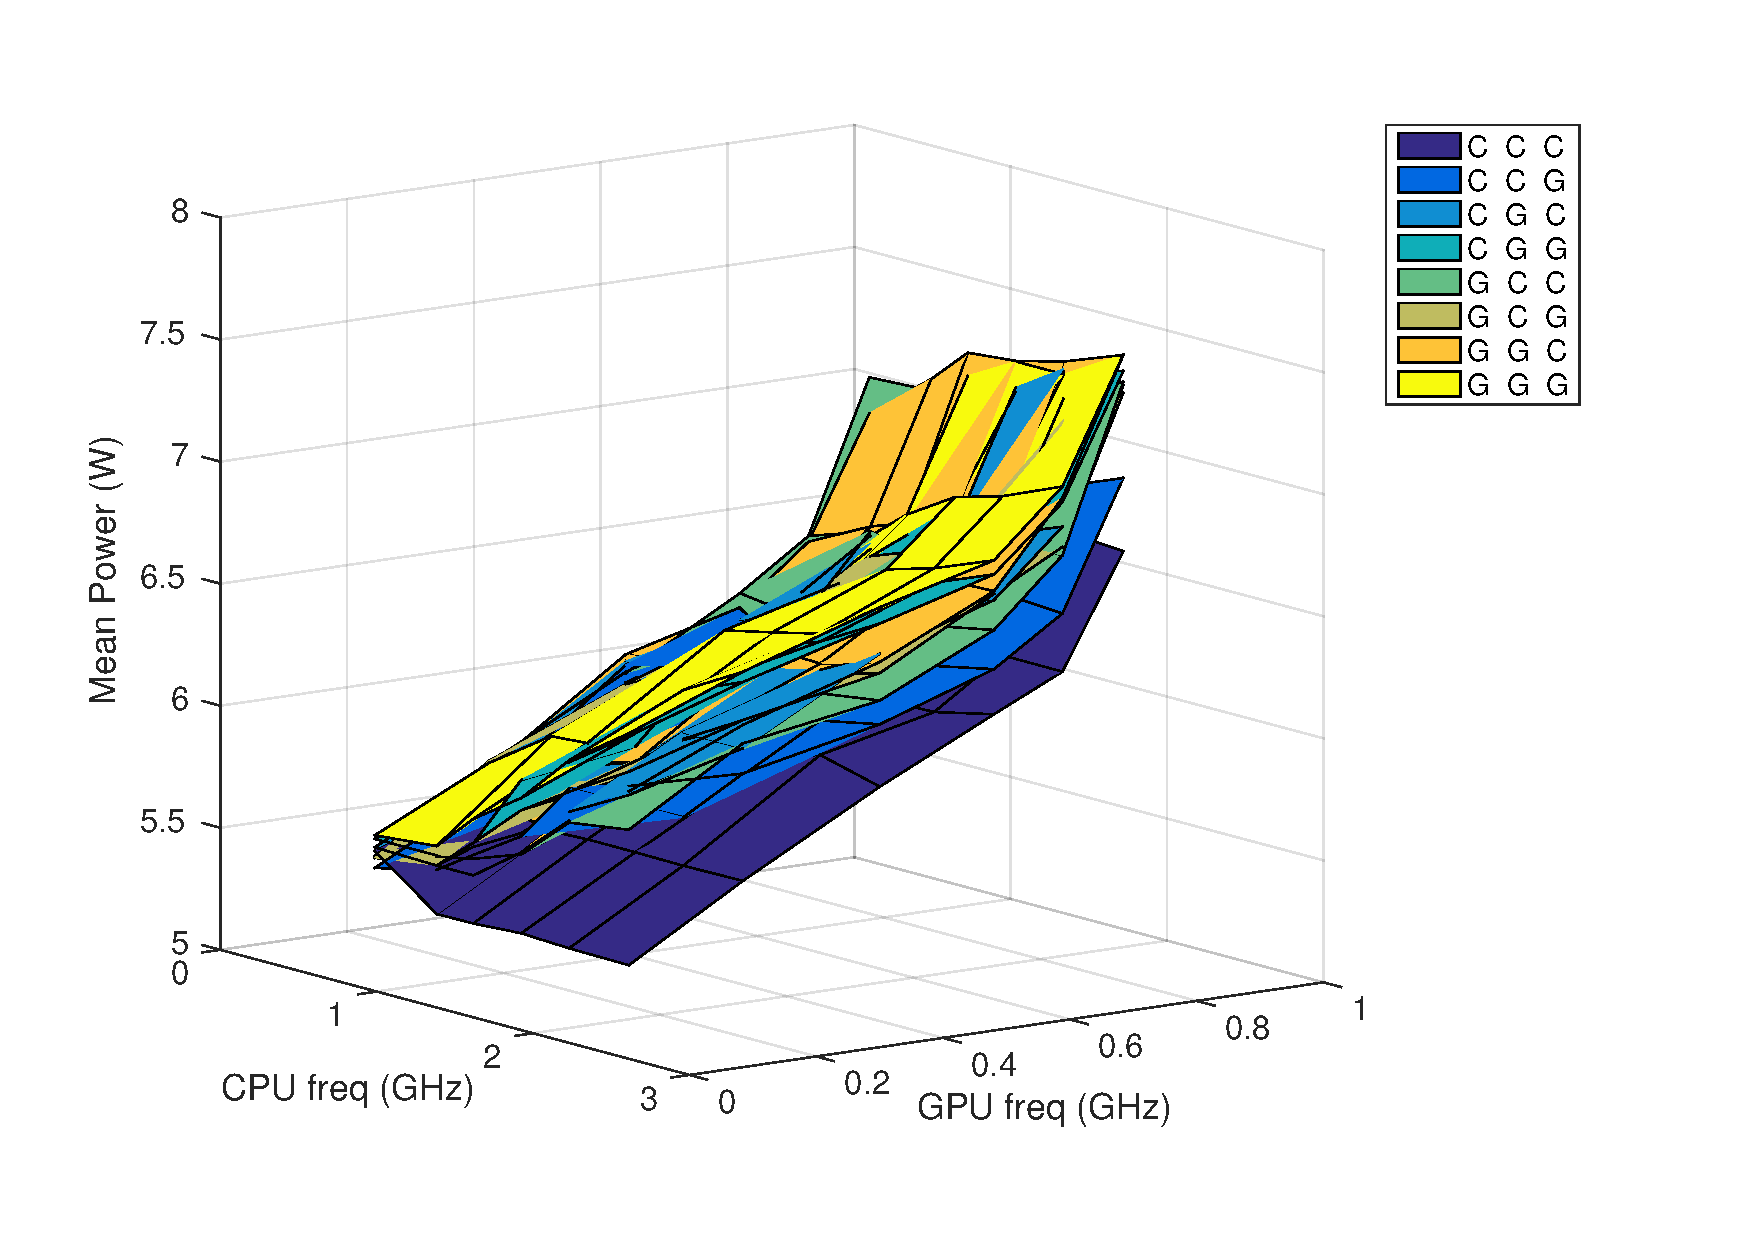
\includegraphics[width=0.46\textwidth]{Figs/surf_Power.pdf}
	\caption{Mean power consumed by the Jetson. Each surface corresponds to a particular schedule (see legend). For a given schedule, different CPU and GPU frequencies yields a different power. (Color in online version).}
	\label{fig:sfda_pow}%same freq diff assignment}
\end{figure}

%\begin{figure}[htbp]
%\centering
%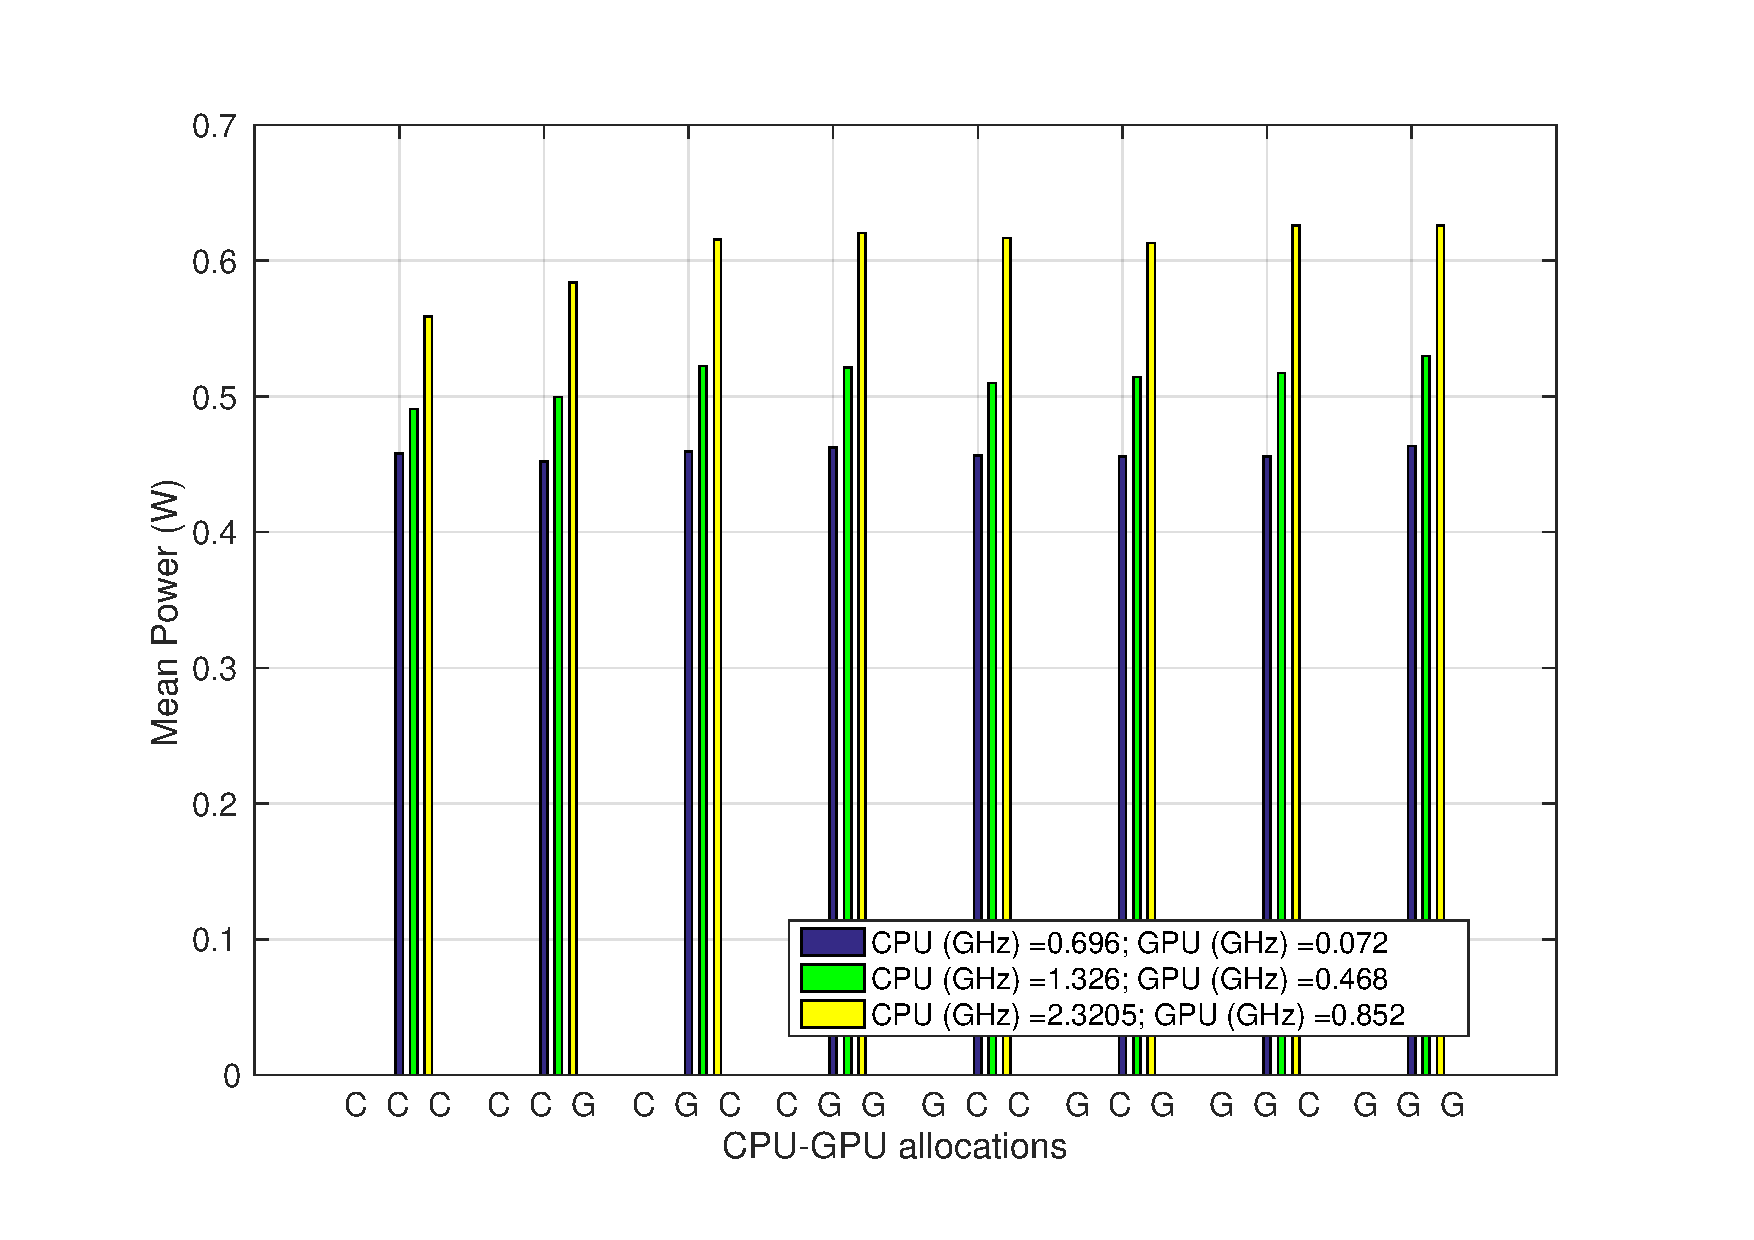
\includegraphics[width=0.46\textwidth]{Figs/PowerHist.pdf}
%\caption{Mean power consumed by the Jetson for different frequencies and a given CPU-GPU assignment.  For clarity we only consider 3 CPU and GPU frequencies for this figure, ranging from the minimum and maximum of both the CPU and the GPU. (Color in online version)}
%\label{fig:dfsa_pow} %diff freq same assignment}
%\end{figure}